\subsection{Matrix Multiplication}
Matrix multiplication is a critical operation in many machine learning algorithms, particularly in the domain of deep learning. Training parameters (weights) of a deep neural network in a vectorized fashion essentially involves multiplication of matrices with various sizes. 

Fully-Connected (FC) layers (Fig.~\ref{fig:fc}) and convolutional (Conv) layers (Fig.~\ref{fig:cnn}) are building blocks of feed-forward and convolutional neural networks~\cite{Warden15}. It is straightforward to identify matrix multiplication in computing output value of a FC layer: each input has $k$ elements, and FC layer has $n$ neurons each with $k$ weights. An FC layer is the multiplication of a $m \times k$ matrix ($m$ is sample size) and a $k\times n$ matrix. A Conv layer appears to be a specialized operation, but it can be computed with matrix multiplication after rearranging data in a matrix format: each depth-wise (channel) slice of input can be added into an input matrix as a row; similarly each kernel can be added into a kernel matrix as a column. Convolution operation becomes multiplication of those two matrices. When using AlexNet on image classification with ImageNet dataset, vast majority of computation time on forward pass (94.7\% on GPU, and 88.7\% on CPU) is consumed by Conv and FC layers~\cite{Jia14}.

\begin{figure}[t]
    \centering
    \begin{subfigure}[b]{0.2\textwidth}
    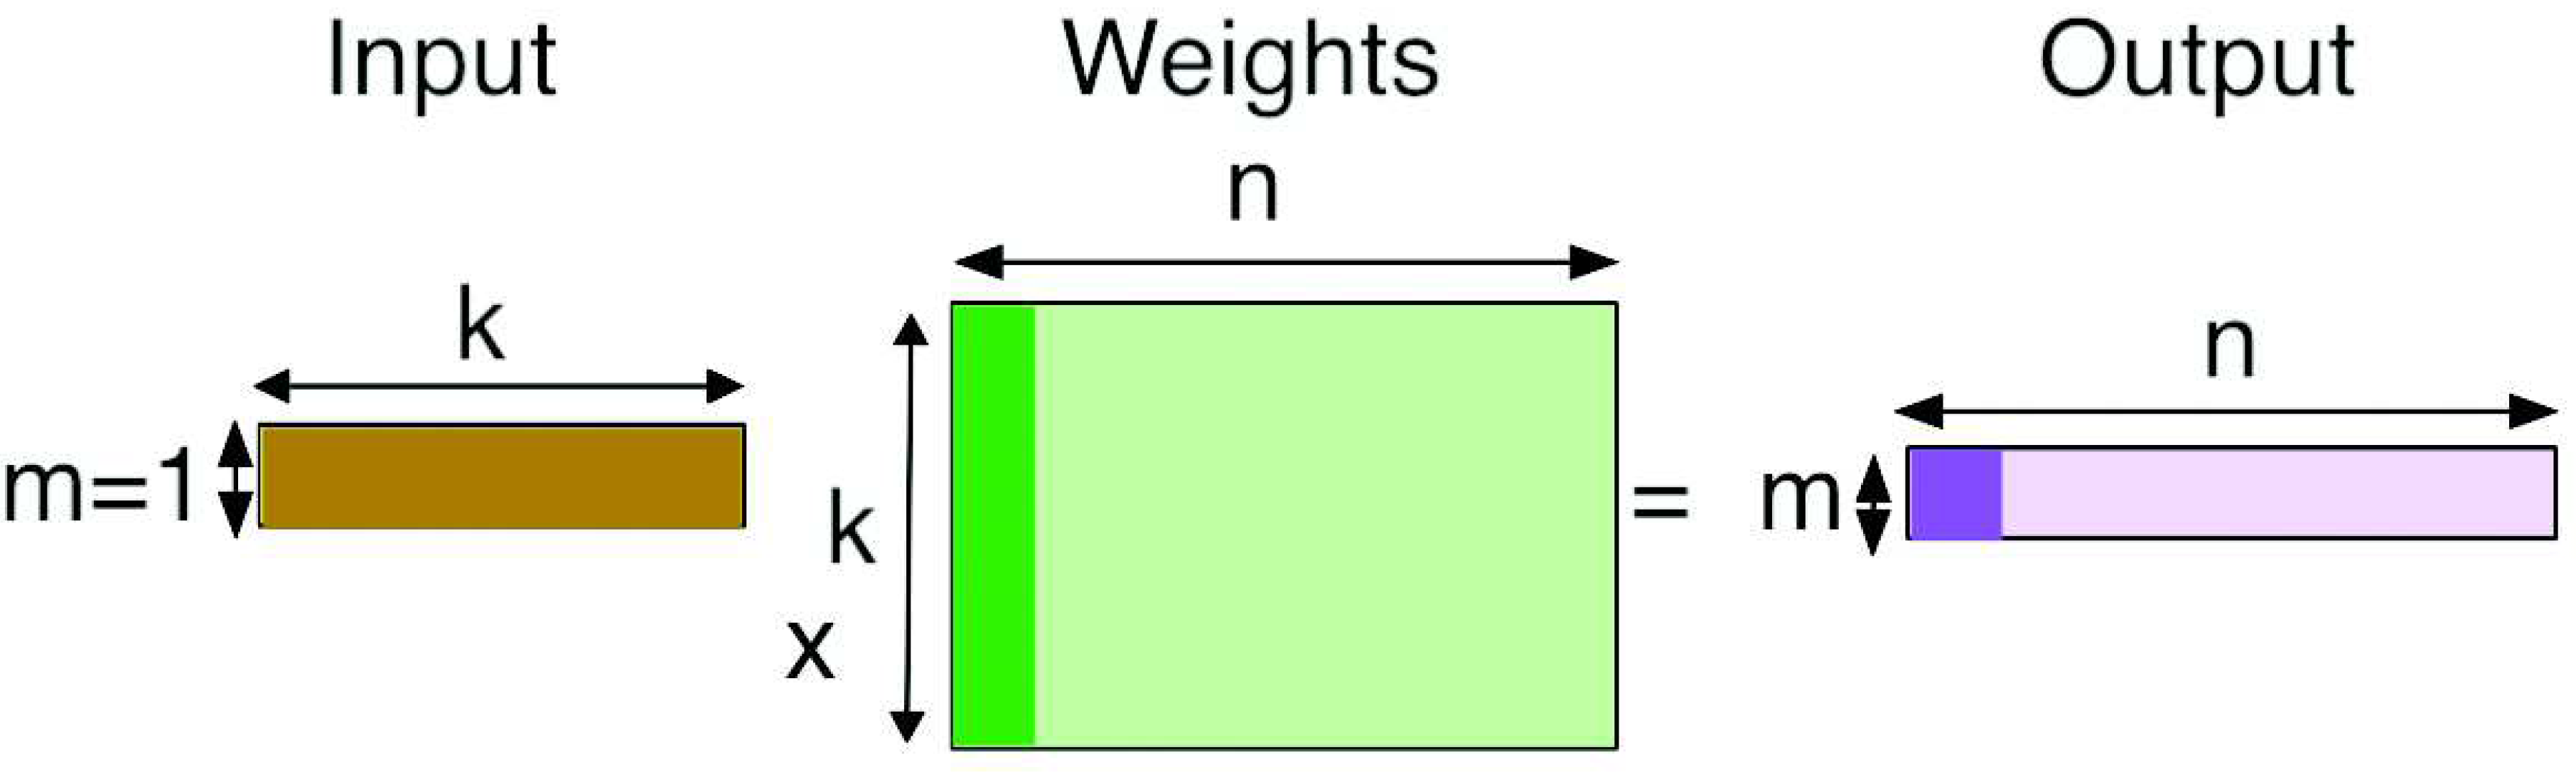
\includegraphics[width=\linewidth]{3_GEMM_backgrounds/fc.png}
    \caption{Fully-Connected Layer}
    \label{fig:fc}
    \end{subfigure}
    \hspace{0.2in}
    \begin{subfigure}[b]{0.2\textwidth}
    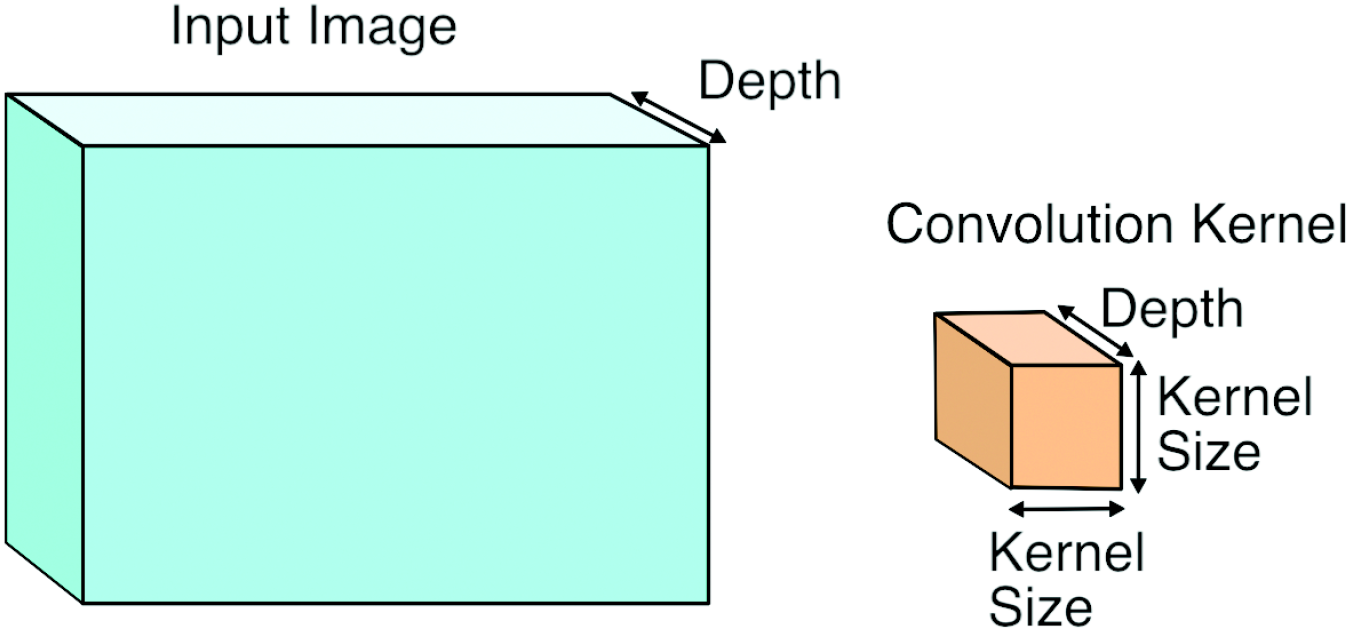
\includegraphics[width=\linewidth]{3_GEMM_backgrounds/cnn.png}
    \caption{Convolutional Layer}
    \label{fig:cnn}
    \end{subfigure}
    \caption{Illustration of deep neural network layers}
    \label{fig:layers}
\end{figure}


% \begin{figure}[h]
%     \vspace{-0.5in}
%     \centering
%     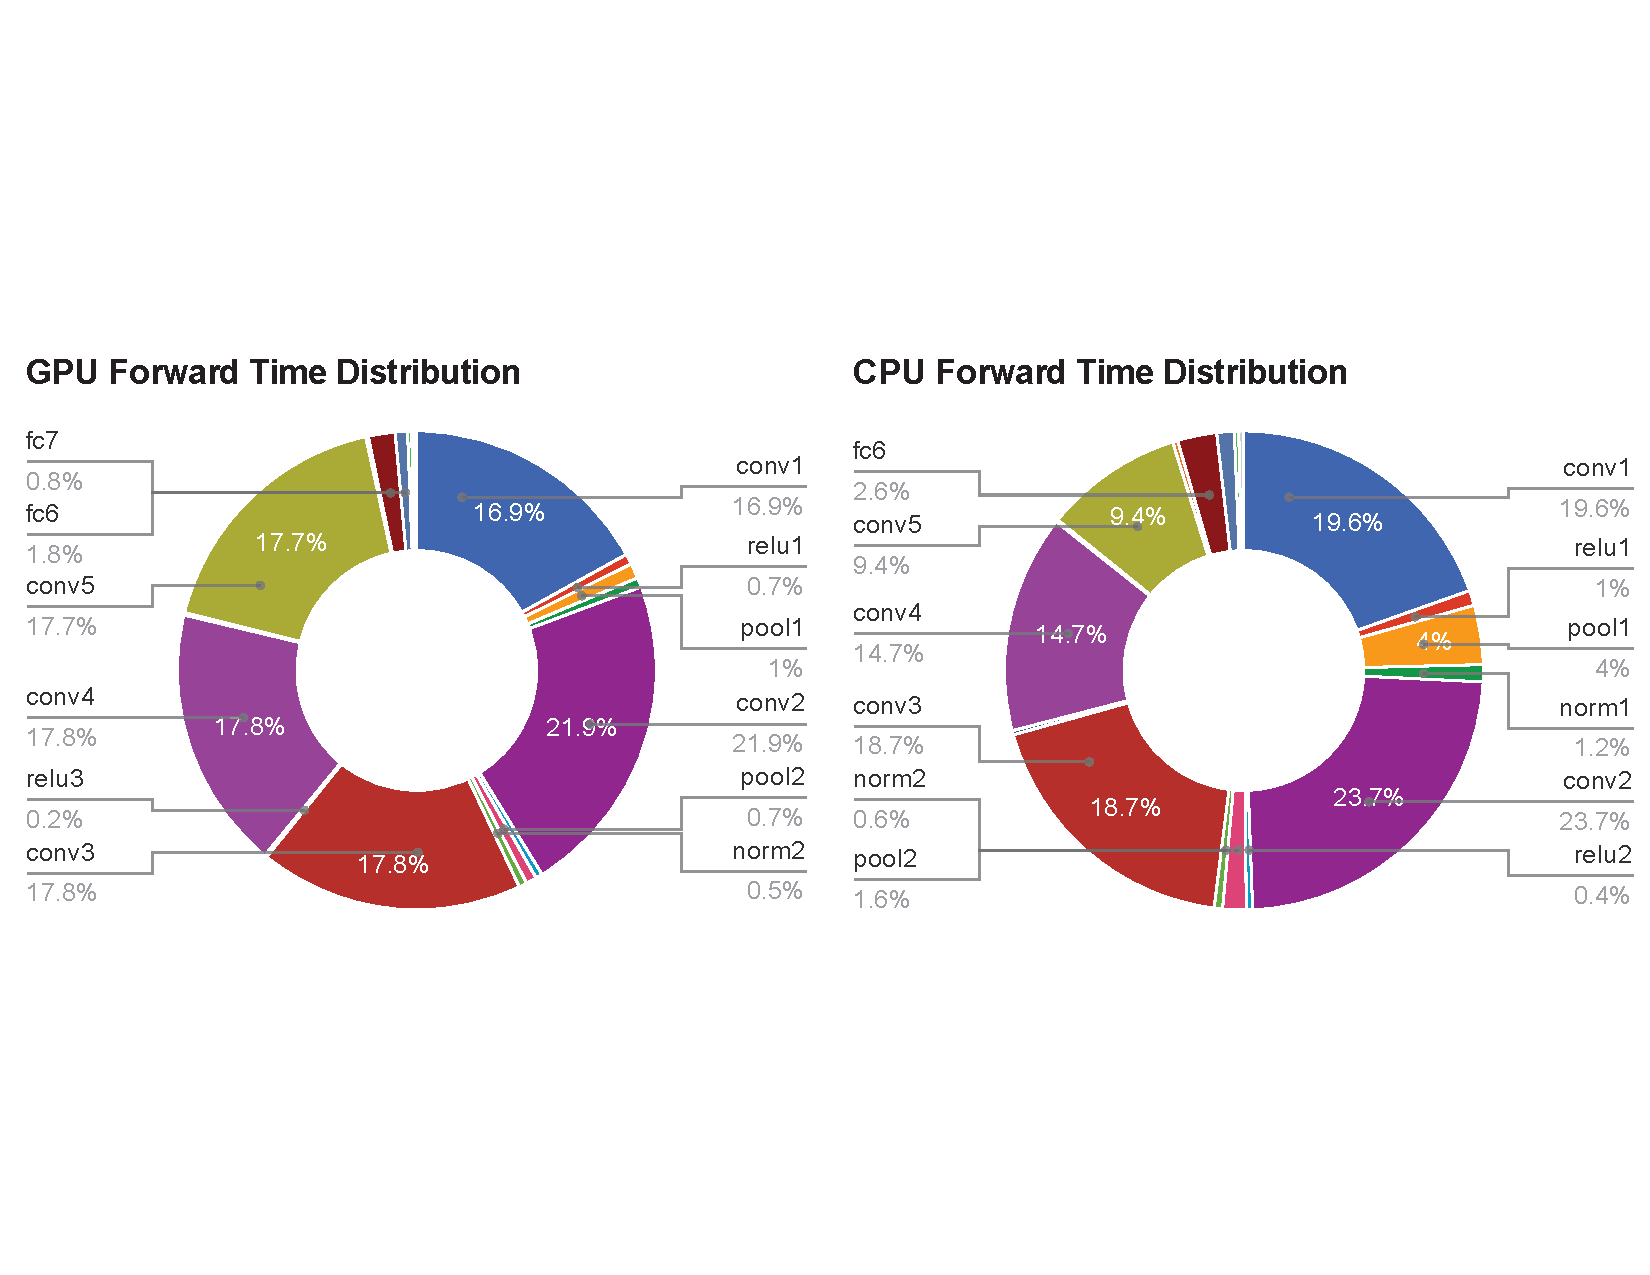
\includegraphics[width=3.2in]{3_GEMM_backgrounds/cnn_time_distribution.pdf}
%     \vspace{-0.5in}
%     \caption{Breakdown of CNN computation time}
%     \label{fig:cnn_time}
% \end{figure}

\subsection{GEMM and Matrix Tiling}
%GEneral Matrix Multiplication (GEMM) is initially part of the BLAS (Basic Linear Algebra Subprograms) library \cite{BLAS2002}. It has the following iterative form:
%\begin{equation}
%    C \Leftarrow \alpha AB + \beta C \nonumber.
%\end{equation}

GEMM is a general procedure ubiquitously used in linear algebra, machine learning, statistics, and many other areas and is implemented in the BLAS (Basic Linear Algebra Subprograms) library \cite{BLAS2002}. It multiplies two input matrices to produce an output matrix. The key difference between GEMM in deep learning and regular matrix multiplication is that the input matrices handled in deep learning are normally much larger. For example, a single layer in a typical convolution neural network may require multiplication of a $256 \times 1024$ matrix by a $1024\times 128$ matrix to produce a $256 \times 128$ matrix. Regular three-for-loop (Fig.~\ref{fig:three}) computation requires 34 million ($256 \times 1024 \times 128$) floating point operations (FLOPs). Modern deep neural networks may have hundreds of convolutional layers (e.g. ResNet152~\cite{He15}), and such networks may need several billions of FLOPs to finish operations in all layers for an input image. 

\begin{figure}[h]
    \centering
    \vspace{-0.1in}
    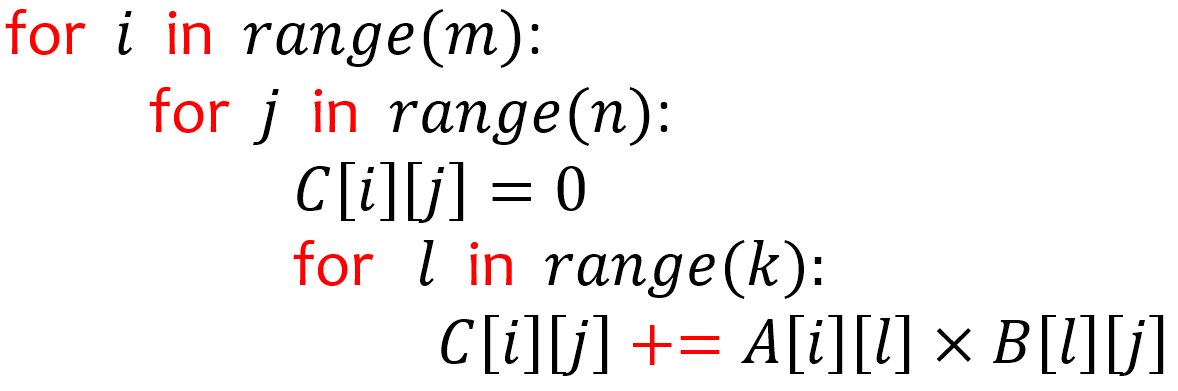
\includegraphics[width=2in]{3_GEMM_backgrounds/three_for_loop.png}
    \vspace{-0.1in}
    \caption{Computing matrix multiplication}
    \label{fig:three}
\end{figure}

High cache hit rate of memory access is critical for complex numerical computation, such as GEMM. The large sizes of matrices usually forbid the entire matrices being loaded into memory or cache, however, GEMM can optimize memory access by iteratively splitting computation into smaller tiles, often referred to as the \emph{tiling process}.
% Large matrices cannot be loaded into memory or cache, so tiling matrices into blocks with GEMM is required to compute large matrix multiplication iteratively.
A resulted matrix is initialized with zeros. GEMM uses outer products to compute part of a tile of the result and accumulates it on top of what has been stored in that tile. A tile is loaded from memory into cache and accumulates a new result on top of that. Fig.~\ref{fig:tiling}~\cite{Matthes17} illustrates a tiling strategy of GEMM.
 
\begin{figure}[t]
  \vspace{-0.5in}
    \centering
    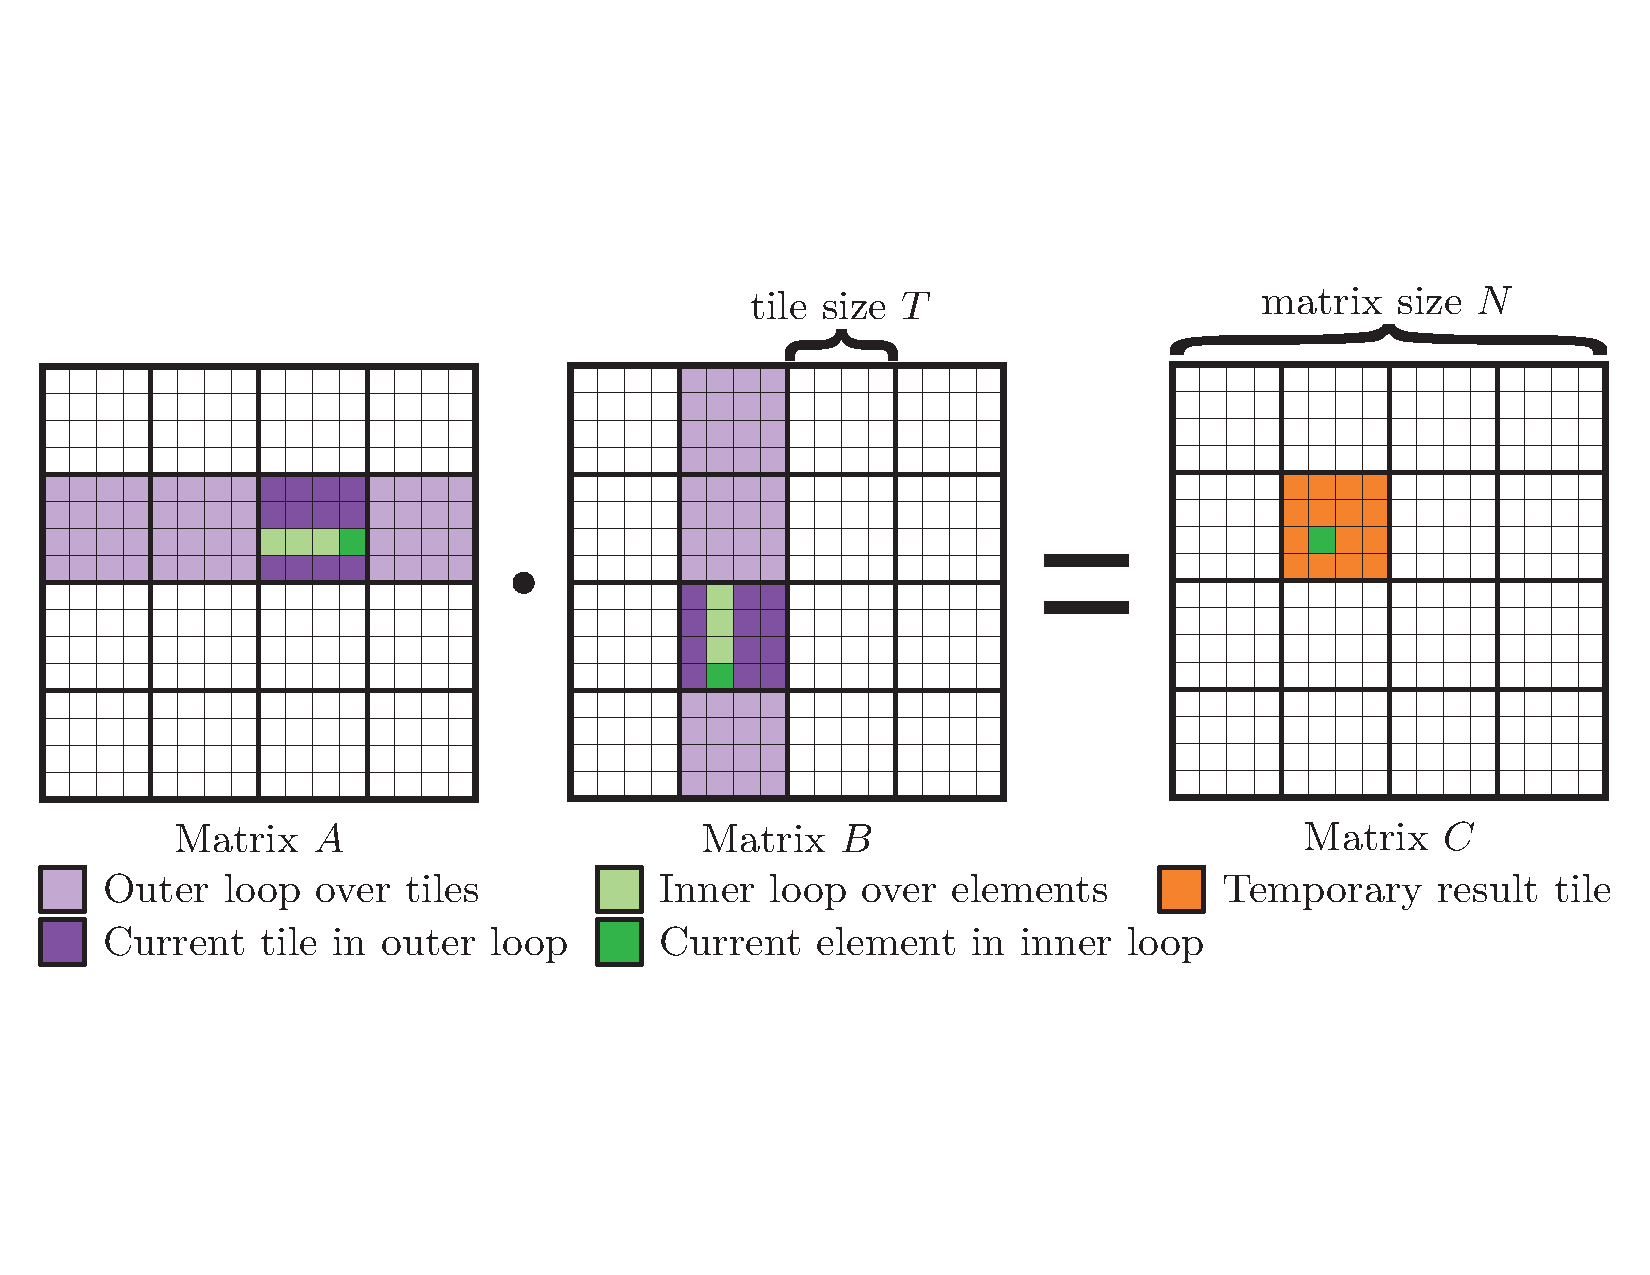
\includegraphics[width=3in]{3_GEMM_backgrounds/tiling.pdf}
    \vspace{-0.5in}
    \caption{An Example of Tiling Strategy}
    \label{fig:tiling}
\end{figure}

Original memory access patterns need to be transformed to adapt to the cache policy of a particular hardware. It is not straightforward to decide an optimal tiling strategy because it requires accurate estimate of accessed array regions in loops to match with cache size of target hardware and meet other constraints. Optimal tiling chooses a tile size for each loop to collectively achieve lowest running time on target hardware.